%!TEX root = /Users/ede/Documents/Master/19_AS/Ausarbeitung/as-ausarbeitung.tex
\section{Tag-Ranking Verfahren} % (fold)
\label{sec:tag_ranking_verfahren}
Hier erfolgt die Darstellung der Tag-Ranking Verfahren im genauen. Und eine bessere Einleitung für dieses Kapitel.

% 
% 
% \begin{itemize}
%   \item   Visual diversification of image search results \cite{diversification}
%   \item   Tag ranking \cite{ranking}
%   \item   Learning to tag \cite{learningToTag}
%   \item   Learning tag relevance by neighbor voting for social image retrieval \cite{learningtagrelevance}
%   \item   Improving recommendation lists through topic diversification \cite{improvingRecommendations}
%   \item   Why we tag: motivations for annotation in mobile and online media \cite{whyWeTag}
%   \item   Flickr tag recommendation based on collective knowledge \cite{collectiveKnowledge}
% \end{itemize}

\subsection{Ranking basierend auf kollektivem Wissen nach Sigurbjörnsson und van Zwol} % (fold)
\label{sub:ranking_basierend_auf_kollektivem_wissen_nach_zwol}

% \begin{itemize}
%   \item Tag co-occurrence is the key to our tag recommendation approach, and only works reliable when a large quantity of supporting data is available.
%   \item 
%   \item Symmetric measures vs. Asymmetric measures
%   \item Zweiter Schritt: Tag Aggregation and Promotion
%   \begin{itemize}
%     \item Aggregation durch \emph{Vote} und \emph{Sum} Verfahren
%     \item Priorisierung der Tags durch \emph{Stability-promotion} und \emph{Descriptiveness-promotion}
%   \end{itemize}
% \end{itemize}



Im Folgenden wird kurz das gesamte Verfahren von \cite{collectiveKnowledge} skizziert und anschließend näher erläutert. Das Verfahren produziert für vom Benutzer vergebene Tags eine geordnete Liste von weiteren, zugehörigen Tags. Grundlage des Rankings ist die \emph{co-occurrence}, oder zu deutsch \emph{gemeinsames Auftreten}, von Tags bei unterschiedlichen Bildern. Diese Häufigkeits-Größe fließt zunächst in die Generierung von einer Kandidaten-Sequenz von zugehörigen Tags für jedes vom Benutzer vergebene Tag ein. Die Sequenz dient dann als Eingabe für die Tag Aggregation und das anschließende Tag Ranking, was die endgültige, nach Relevanz sortierte Liste von Tags ergibt. Abbildung \ref{fig:images_collective_knowledge_system_overview} veranschaulicht das System.

\begin{figure}[htbp]
  \centering
    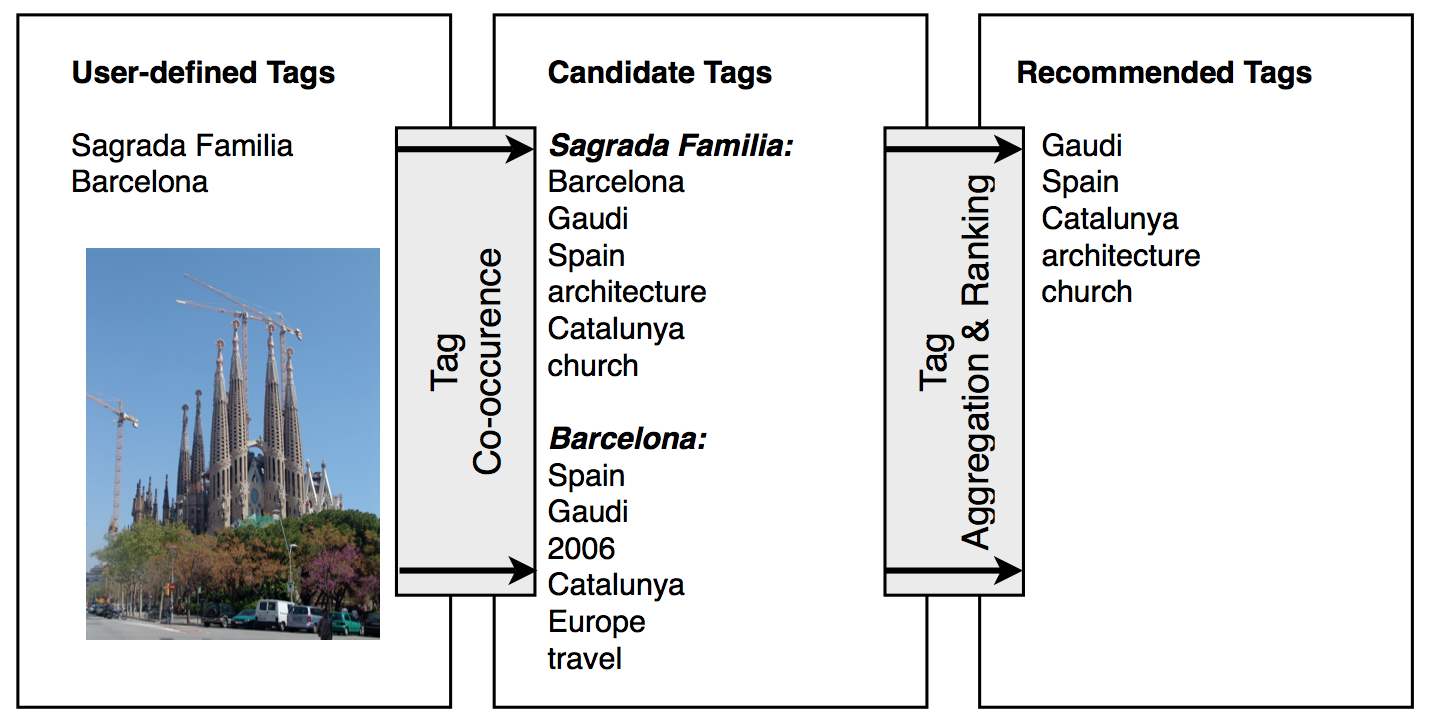
\includegraphics[height=3in]{images/collective_knowledge_system_overview.png}
  \caption{Übersicht des Tag Empfehlungssytems nach \cite{collectiveKnowledge}.}
  \label{fig:images_collective_knowledge_system_overview}
\end{figure}




 % - Verfahren basiert auf Tag co-occurrence
% Tag co-occurrence is the key to our tag recommendation approach, and only works reliable when a large quantity of supporting data is available.

Die mathematische Definition von co-occurrence nach \cite{collectiveKnowledge} lautet \emph{``We define the co-occurrence between two tags to be the number of photos [in our collection] where both tags are used in the same annotation.''}
 
 % - sehr einfache basis für verfahren
 
Um den wert der co-occurrence von der allgemeinen Verwendungsfrequenz der Tags zu trennen, wird dieser Wert normalisiert. Co-occurrence als Maßeinheit für das gemeinsame Auftreten von Tags kann auf unterschiedliche Weise normalisiert werden, was starke Auswirkung auf das Ergebnis hat.

Die symmetrischen Normalisierung gibt die Äquivalenz von zwei Tags, ${t_i}$ und ${t_j}$ an, da hierbei die Summe der Anzahl beider Tags als Divisor verwendet wird und somit die gemeinsame Auftrittswahrscheinlich für diese beiden Tags angegeben wird. Beispielsweise sind zu \emph{Eiffel Tower} als äquivalent gefundene Tags \emph{Tour Eiffel, Eiffel, Seine, La Tour Eiffel} und \emph{Paris}.
\begin{figure}[hptb]
  \begin{equation}
  \label{symmetricNormalization}
   J(t_i, t_j) := \frac{\vert t_i \cap t_j \vert}{ \vert t_i \cup t_j \vert }
  \end{equation}
\end{figure}

Die co-occurrence $J(t_i, t_j)$ ist also ein Koeffizient aus der Schnittmenge der Tags ${t_i}$ und ${t_j}$, und der Vereinigungsmenge von ${t_i}$ und ${t_j}$.

Bei der asymmetrischen Normalisierung wird die Anzahl des gemeinsamen Auftretens durch die Anzahl des ersten Tags dividiert. Damit wird also erfasst, wie oft ${t_i}$ gemeinsam mit ${t_j}$ gelistet wird, was beim Vorschlagen von tags mehr Sinn macht, damit der Inhalt der Photos möglichst vielfältig anstatt genau getaggt werden kann. So ergibt der Tag \emph{Eiffel Tower} folgende Sequenz assoziierter Tags: \emph{Paris, France, Tour Eiffel, Eiffel} und \emph{Europe}.
   % TODO: hier gibts kritikmöglichkeit, warum diese normaliesierung gewählt wurde, evtl. später aufgreifen.
\begin{figure}[hptb]
 \begin{equation}
 \label{asymmetricNormalization}
  J(t_i \vert t_j) := \frac{\vert t_i \cap t_j \vert}{ \vert t_i \vert }
 \end{equation}
\end{figure}

In Anbetracht der Aufgabe, die Medien möglichst vielfältig zu Taggen, wird die zweite Varianten von den Autoren verwendet.

Bei der Aggregation werden die Kandidaten-Sequenzen für die unterschiedlichen vom Benutzer vergebenen Tags zu einer einzigen geordneten Liste zu vereinigen. Dabei werden zwei unterschiedliche Strategien vorgeschlagen, denen Gemeinsamkeit darin besteht, dass sie jeweils über alle Kandidaten-Tags iterieren. Die erste wertet Tags höher, die in allen Kandidaten-Sequenzen vorkommen, die zwei betrachtet nur den Wert der co-occurrence für die Tags.

Hier folgen noch die mathematischen Erläuterungen.

Anschließend fließen die Untersuchungsergebnisse aus Kapitel \ref{sec:analyse_und_klassifikation}, dass sehr oft benutzte Tags wenig aussagefähig sind sowie dass sehr selten benutzte Tags zu spezifisch sind, in den Ranking Schritt ein. Die \emph{Descriptiveness-promotion} wertet Tags mit sehr hoher Frequenz ab. Das als \emph{Stability-promotion} bezeichnete Ranking reduziert den Ranking Wert bei geringer Frequenz. So werden alle Tags in Relation zu ihrer Verwendungshäufigkeit bewertet.

Hier folgen noch die mathematischen Erläuterungen.

Der eben gelesene Abschnitt zum Verfahren von \cite{collectiveKnowledge} wird noch weiter vertieft werden.

% subsection ranking_basierend_auf_kollektivem_wissen_nach_zwol (end)

\subsection{Verbesserung der Relevanz von Tags durch einen Random Walk nach Liu u. a.} % (fold)
\label{sub:verbesserung_der_relevanz_durch_einen_random_walk}

% \begin{itemize}
%   \item Wahrscheinlichkeitsorientierte Schätzung der Relevanz von Tags.
%   \item Random-Walk basierte Verfeinerung des Rankings
%     
%     \begin{itemize}
%       \item Aufbau eines Beziehungs-Graphen der Tags.
%       \item Random Walk über den Graphen
%     \end{itemize}
% \end{itemize}

% Bei diesem Verfahren wird wie bei dem von \cite{collectiveKnowledge} die co-occurrence als Initialwert für den Rank eines Tags gewählt.
- Initialwert ist zunächst für alle Tags gleich

- Zunächst Bestimmung des Wertes durch Beziehung zu Photos mit gleichen Tags, ähnliche dem Ansatz von \cite{collectiveKnowledge}. Dieser Wert ist die Gewichtung der Kanten zwischen zwei Tags/Knoten im folgenden Graph.

- Daraufhin wird ein Tag Graph erstellt, der als Basis für einen Random Walk dient. Vgl. \cite{} für Random Walk Literatur. 

- Dabei wird der Graph als Matrix mit den Ranking Werten formuliert. 

- Durch den Random Walk werden die Relevanzwerte durch die Gewichtung der Tags zu einander angepasst.
% Initialwert für den Rank eines Tags wird durch die Beziehung zwischen durch die Photos assoziierten Tags bestimmt. Für jedes Photo x mit den Nachbarn (haben den gleichen Tag) X

% Daraufhin erfolgt das Erstellen eines Tag Graphen 



\begin{figure}[htbp]
  \centering
    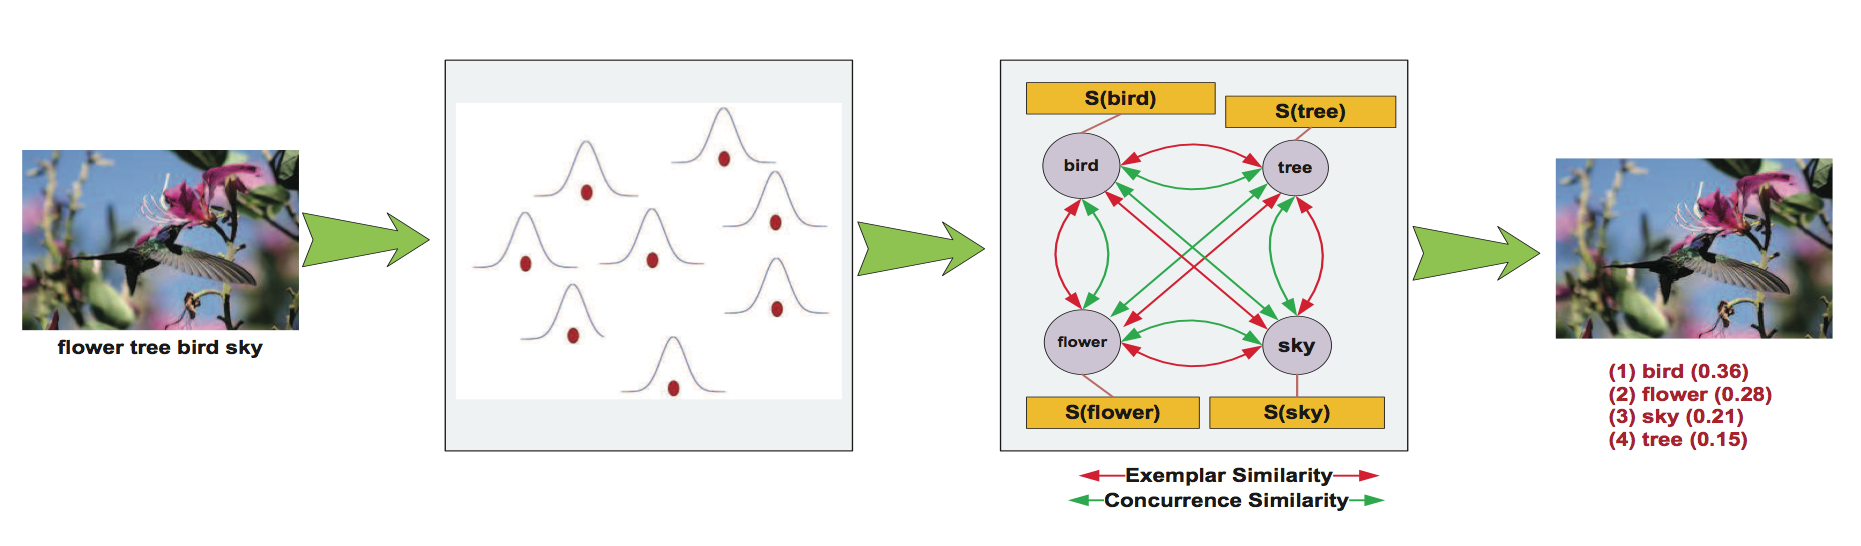
\includegraphics[height=2in]{images/tag_ranking_verfahren.png}
  \caption{Schema zum Tag Ranking Ansatz von \cite{ranking}.}
  \label{fig:images_tag_ranking_verfahren}
\end{figure}


Dieses Verfahren wird ähnlich dem obigen und zu gegebener Zeit erläutert werden :)

% subsection verbesserung_der_relevanz_durch_einen_random_walk (end)
% section tag_ranking_verfahren (end)
